\documentclass[10pt,a4paper]{article}
\usepackage[utf8]{inputenc}
\usepackage[T1]{fontenc}
\usepackage[spanish]{babel}
\usepackage{geometry}
\usepackage{graphicx}
\usepackage{booktabs}
\usepackage{float}
\geometry{margin=2.2cm}
\graphicspath{{../../../../results/figures/}}
\setlength{\parskip}{0.5em}
\setlength{\parindent}{0pt}

\title{Informe técnico de optimización, regularización y evaluación final\\Fashion-MNIST}
\author{Cesar Rojas}
\date{20 de septiembre de 2026}

\begin{document}
\maketitle

\section{Alcance y protocolo}

Esta etapa recibe como control la MLP $[256,128]$, ReLU, Softmax, categorical crossentropy, SGD con learning rate 0,1, batch 128, 20 épocas y seed 42. El objetivo es estudiar optimizadores y regularización mediante experimentos controlados, congelar una configuración usando solo validation y evaluar test una única vez.

Se conservó el split estratificado de 54.000 ejemplos de train y 6.000 de validation. El test oficial permaneció sellado durante E6--E9. Las decisiones usan Accuracy, F1 Macro, curvas de validation y gaps train--validation; test se consulta solamente después de F0.

\section{E6 y E6b: optimizadores}

E6 cambió únicamente el optimizador bajo learning rate común 0,1. SGD fue el control más estable; el rendimiento bajo de Adam y RMSProp no se interpretó como una descalificación general, sino como evidencia de que esa escala de LR no era adecuada. E6b cambió solamente el LR de cada adaptativo a 0,001.

\begin{table}[H]
\centering
\begin{tabular}{llrrrr}
\toprule
ID & Optimizador / LR & Accuracy & F1 Macro & Gap acc. & Gap loss \\
\midrule
E6 & SGD / 0,1 & \textbf{0,8952} & \textbf{0,8954} & \textbf{0,0287} & \textbf{0,0851} \\
E6 & RMSProp / 0,1 & 0,1985 & 0,0684 & --- & --- \\
E6 & Adam / 0,1 & 0,4722 & 0,4166 & --- & --- \\
E6b & Adam / 0,001 & 0,8912 & 0,8916 & 0,0527 & 0,1941 \\
E6b & RMSProp / 0,001 & 0,8933 & 0,8929 & 0,0476 & 0,2165 \\
\bottomrule
\end{tabular}
\caption{E6 y E6b sobre validation.}
\end{table}

SGD conserva la mejor Accuracy y F1 Macro, además de gaps menores que los optimizadores retuneados. Se seleccionó como control provisional para E7; todavía no se usó test ni se congeló la configuración.

\begin{figure}[H]
\centering
\begin{minipage}{.48\linewidth}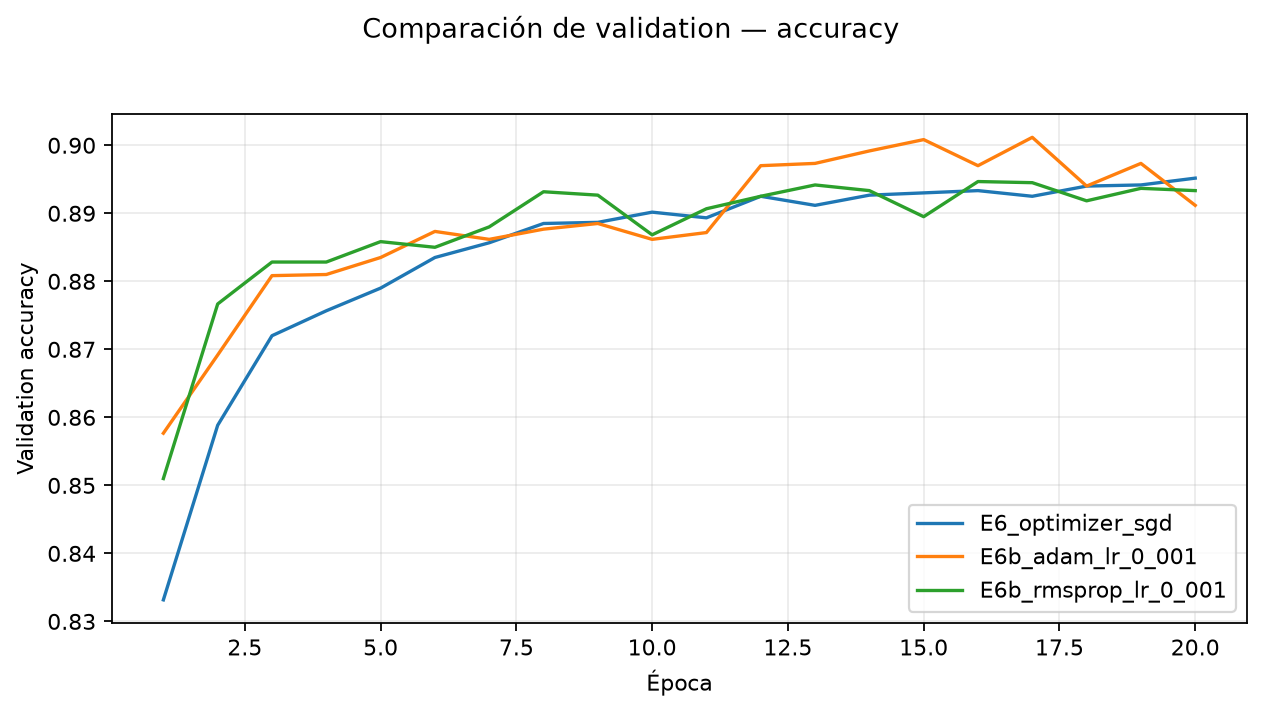
\includegraphics[width=\linewidth]{E6b_retuned_optimizer_validation_accuracy.png}\end{minipage}\hfill
\begin{minipage}{.48\linewidth}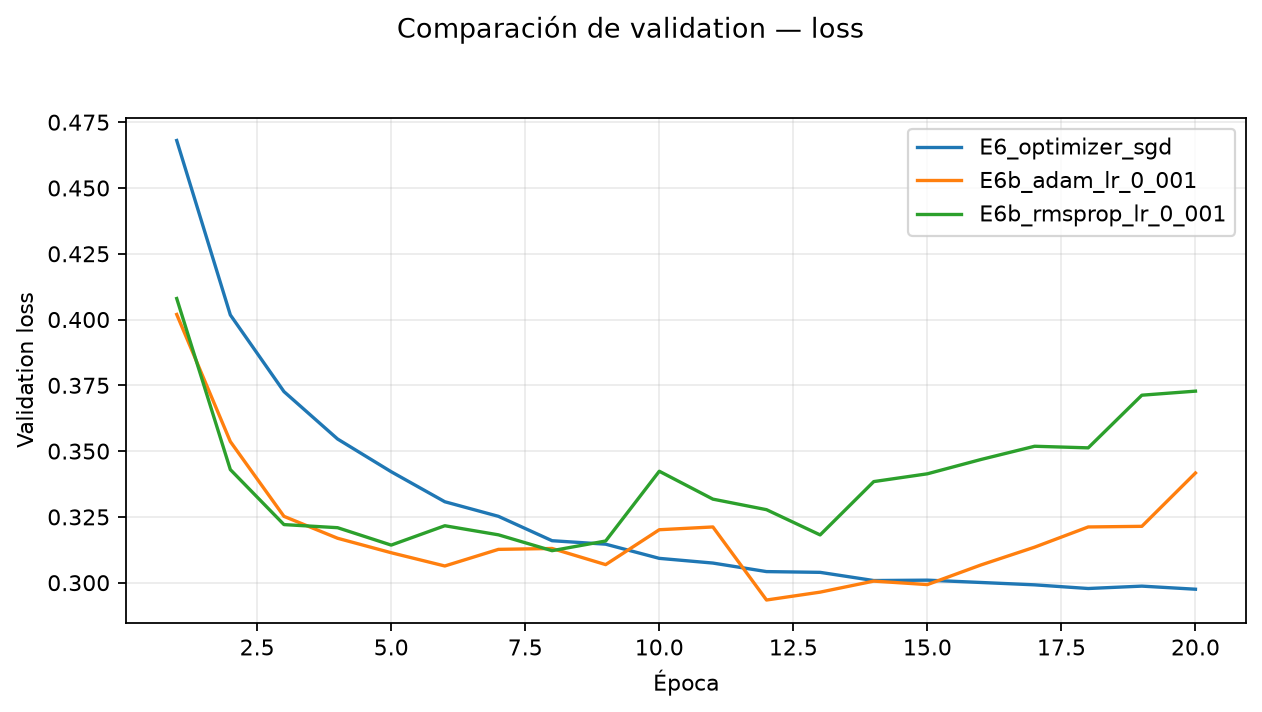
\includegraphics[width=\linewidth]{E6b_retuned_optimizer_validation_loss.png}\end{minipage}
\caption{Curvas de validation para E6b.}
\end{figure}

\section{E7--E9: regularización}

E7 varía exclusivamente Dropout. E8 cambia únicamente Batch Normalization y aplica el orden Dense lineal $\rightarrow$ Batch Normalization $\rightarrow$ ReLU $\rightarrow$ Dropout. E9 cambia solamente la fuerza L2. De esta forma no se atribuyen a una técnica efectos que puedan corresponder a otra.

\begin{table}[H]
\centering
\begin{tabular}{llrrrr}
\toprule
Etapa & Cambio único & Accuracy & F1 Macro & Gap acc. & Gap loss \\
\midrule
E7 & Dropout 0,0 & 0,8952 & 0,8954 & 0,0287 & 0,0851 \\
E7 & Dropout 0,2 & \textbf{0,8997} & \textbf{0,8997} & \textbf{0,0021} & 0,0135 \\
E8 & BatchNorm OFF & \textbf{0,8997} & \textbf{0,8997} & \textbf{0,0021} & \textbf{0,0135} \\
E8 & BatchNorm ON & 0,8922 & 0,8911 & 0,0294 & 0,0827 \\
E9 & L2 0 & \textbf{0,8997} & \textbf{0,8997} & \textbf{0,0021} & 0,0135 \\
E9 & L2 $10^{-4}$ & 0,8967 & 0,8970 & 0,0025 & \textbf{0,0102} \\
\bottomrule
\end{tabular}
\caption{Comparaciones controladas de regularización.}
\end{table}

Dropout 0,2 mejoró simultáneamente Accuracy/F1 y generalización, por lo que se seleccionó. Batch Normalization no compensó su costo ni sus gaps mayores en este régimen. L2 redujo marginalmente el gap de loss, pero no mejoró Accuracy ni F1 y su loss incorpora la penalización. Estos dos resultados negativos son contextuales: no afirman que BatchNorm o L2 sean inútiles en general.

\begin{figure}[H]
\centering
\begin{minipage}{.48\linewidth}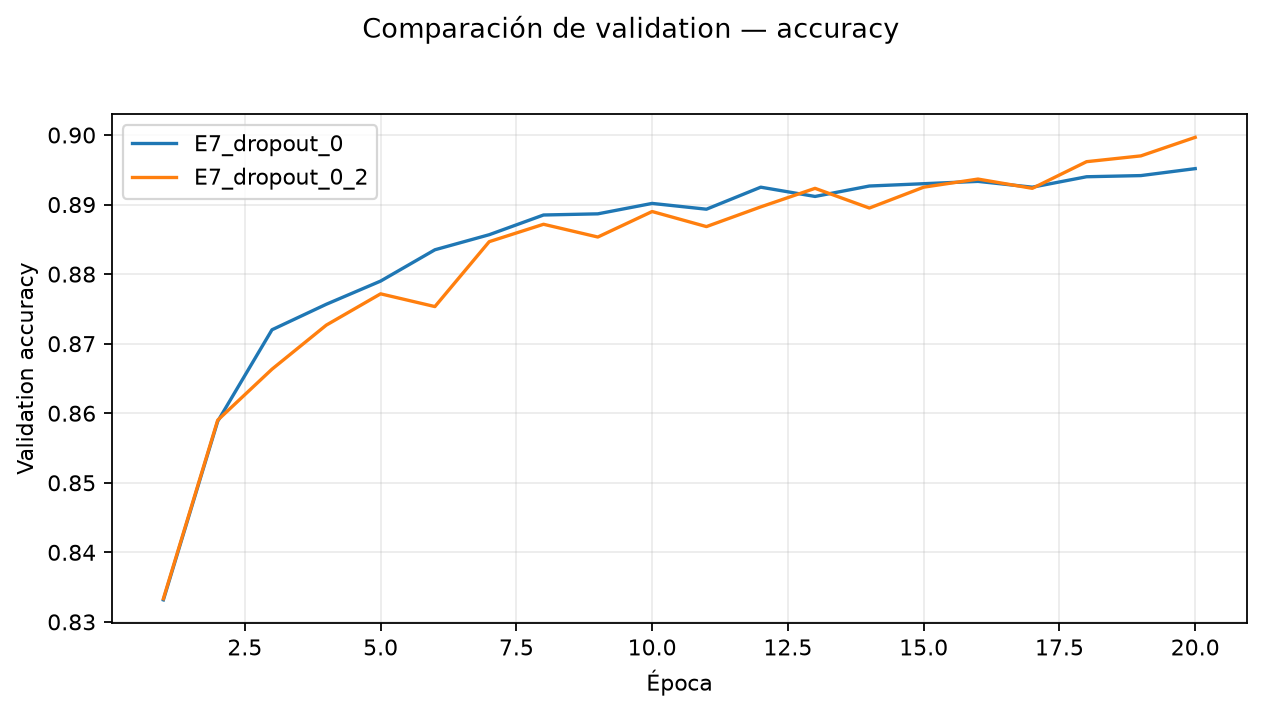
\includegraphics[width=\linewidth]{E7_dropout_validation_accuracy.png}\end{minipage}\hfill
\begin{minipage}{.48\linewidth}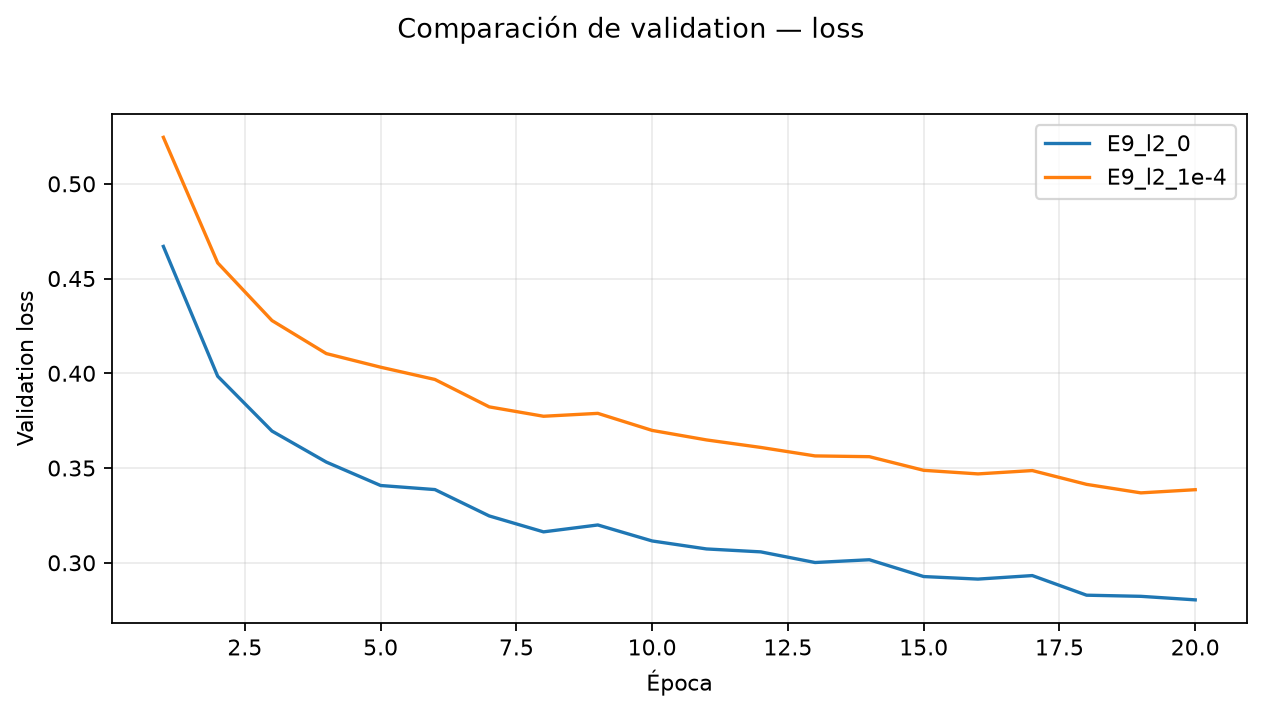
\includegraphics[width=\linewidth]{E9_l2_validation_loss.png}\end{minipage}
\caption{Curvas de validation que respaldan las decisiones E7 y E9.}
\end{figure}

\section{F0: congelamiento}

La decisión L2 se repitió con seed 7: sin L2 obtuvo Accuracy 0,8902 frente a 0,8863 con L2 $10^{-4}$. Con ambas seeds, los promedios fueron 0,8949 sin L2 y 0,8915 con L2. Early Stopping no se implementó porque el control alcanzó su mejor validation accuracy y loss al final de las 20 épocas, sin deterioro sostenido ni ahorro material.

Por tanto, F0 congeló la MLP $[256,128]$, ReLU, Softmax, categorical crossentropy, SGD LR 0,1, batch 128, 20 épocas, seed 42, Dropout 0,2 y sin Batch Normalization, L2 ni Early Stopping. Después de esta decisión no se ajustó ningún parámetro tras observar test.

\section{F1: evaluación final única}

La configuración congelada se entrenó con train 54.000/validation 6.000 y se evaluó una única vez sobre los 10.000 ejemplos oficiales de test.

\begin{table}[H]
\centering
\begin{tabular}{lr}
\toprule
Métrica & Test \\
\midrule
Accuracy & 0,8838 \\
Precision Macro & 0,8844 \\
Recall Macro & 0,8838 \\
F1 Macro & 0,8836 \\
Precision ponderada & 0,8844 \\
Recall ponderado & 0,8838 \\
F1 ponderado & 0,8836 \\
\bottomrule
\end{tabular}
\caption{Métricas globales de F1.}
\end{table}

La matriz de confusión evidencia dificultades entre prendas superiores visualmente similares. Shirt fue la clase más difícil (Precision 0,7021, Recall 0,6930 y F1 0,6975), seguida de confusiones entre T-shirt/top, Pullover y Coat. Esta observación se comunica como limitación y no se usa para modificar el modelo.

\begin{figure}[H]
\centering
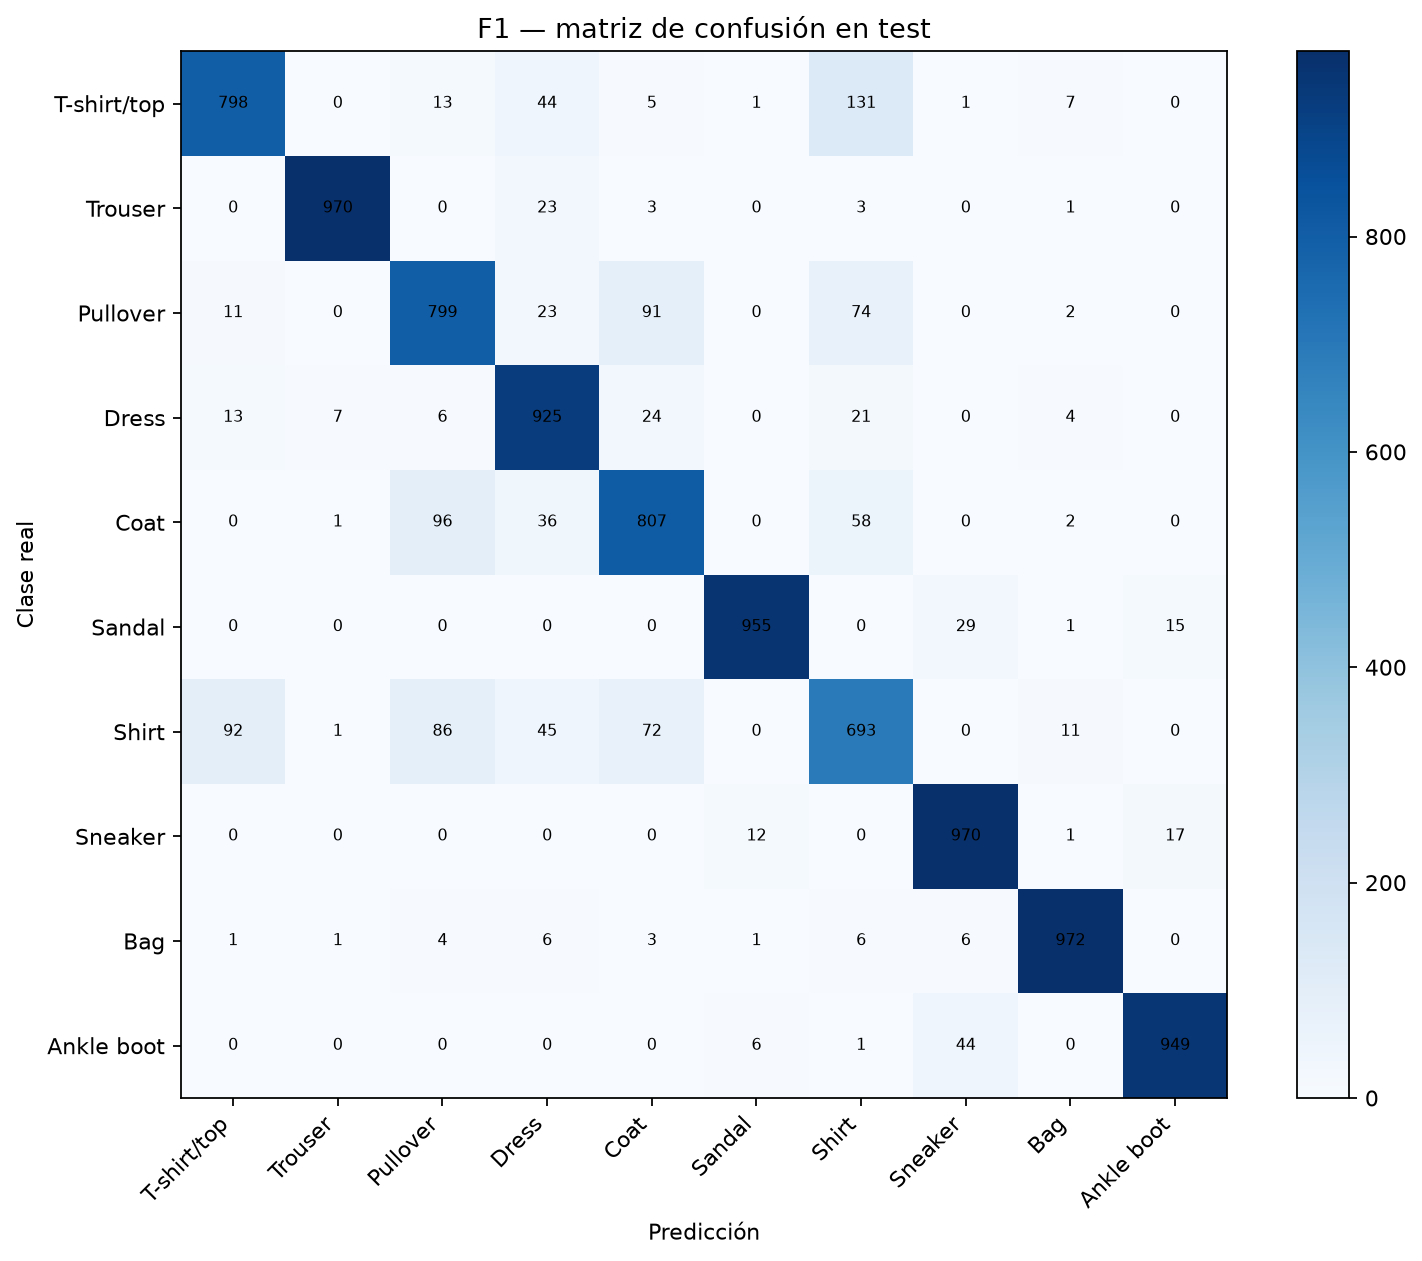
\includegraphics[width=.9\linewidth]{F1_test_confusion_matrix.png}
\caption{Matriz de confusión final sobre test.}
\end{figure}

\begin{figure}[H]
\centering
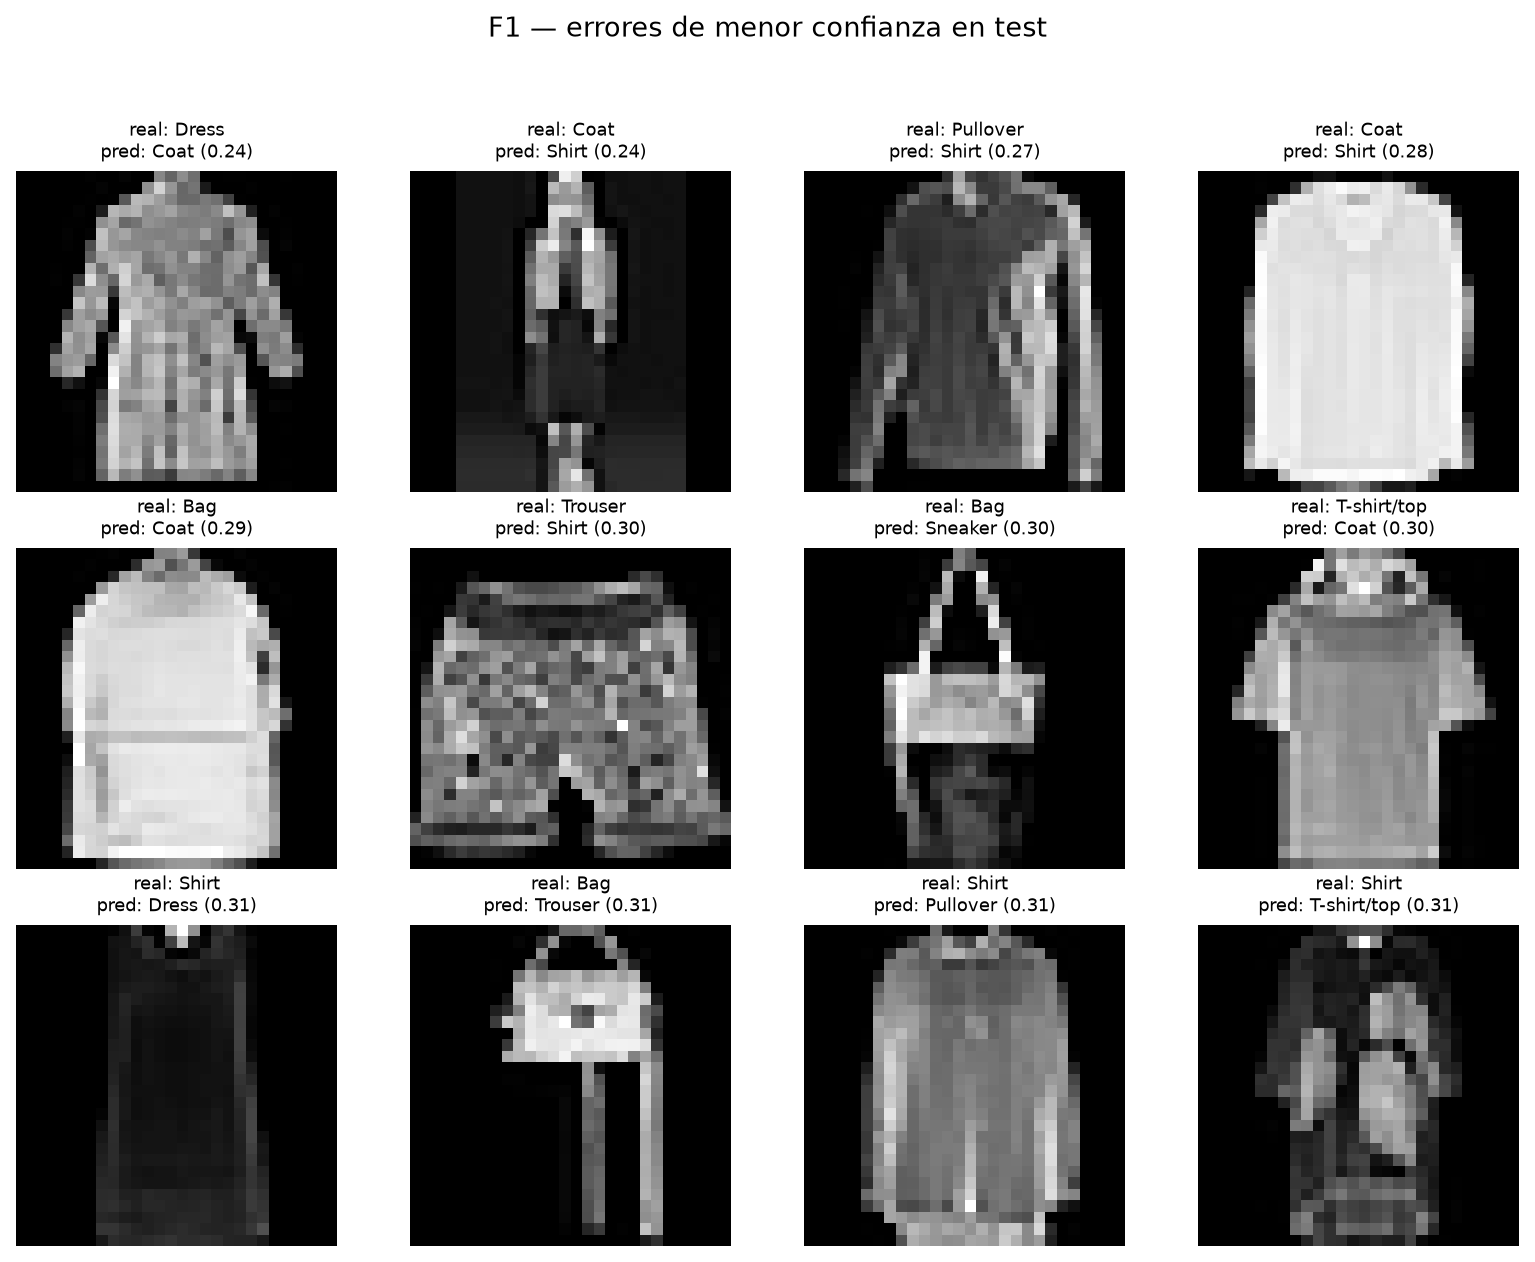
\includegraphics[width=.85\linewidth]{F1_test_low_confidence_errors.png}
\caption{Ejemplos de errores de menor confianza.}
\end{figure}

\section{Conclusión y reproducibilidad}

La etapa demuestra que Dropout 0,2 aportó la mejora de generalización más clara bajo el control recibido. SGD LR 0,1 mantuvo el mejor compromiso ante los optimizadores estudiados, mientras que BatchNorm y L2 no mejoraron las métricas en este régimen. La evaluación final obtuvo Accuracy 0,8838 y F1 Macro 0,8836 sin retroalimentar ajustes desde test.

El código reutilizable, las configuraciones, tablas y figuras se mantienen en el repositorio. La versión final pasa 31 pruebas automatizadas y Ruff. El informe consolidado de las tres etapas se encuentra en \texttt{docs/latex/final/main.tex}.

\end{document}
